% $Id: template.tex 11 2007-04-03 22:25:53Z jpeltier $

\documentclass{vgtc}                          % final (conference style)
%\documentclass[review]{vgtc}                 % review
%\documentclass[widereview]{vgtc}             % wide-spaced review
%\documentclass[preprint]{vgtc}               % preprint
%\documentclass[electronic]{vgtc}             % electronic version
\let\ifpdf\relax

%% Uncomment one of the lines above depending on where your paper is
%% in the conference process. ``review'' and ``widereview'' are for review
%% submission, ``preprint'' is for pre-publication, and the final version
%% doesn't use a specific qualifier. Further, ``electronic'' includes
%% hyperreferences for more convenient online viewing.

%% Please use one of the ``review'' options in combination with the
%% assigned online id (see below) ONLY if your paper uses a double blind
%% review process. Some conferences, like IEEE Vis and InfoVis, have NOT
%% in the past.

%% Figures should be in CMYK or Grey scale format, otherwise, colour 
%% shifting may occur during the printing process.

%% These three lines bring in essential packages: ``mathptmx'' for Type 1 
%% typefaces, ``graphicx'' for inclusion of EPS figures. and ``times''
%% for proper handling of the times font family.

\usepackage{mathptmx}
\usepackage{graphicx}
\usepackage{times}

%% Packages used by us
\usepackage{color}
\usepackage{caption}
\usepackage{subcaption}
\usepackage{tabularx}
\usepackage[normalem]{ulem}

%% Useful definitions
\def\tweakedsim{\raise.17ex\hbox{$\scriptstyle\sim$}}

%% We encourage the use of mathptmx for consistent usage of times font
%% throughout the proceedings. However, if you encounter conflicts
%% with other math-related packages, you may want to disable it.

%% If you are submitting a paper to a conference for review with a double
%% blind reviewing process, please replace the value ``0'' below with your
%% OnlineID. Otherwise, you may safely leave it at ``0''.
\onlineid{1519}

%% declare the category of your paper, only shown in review mode
\vgtccategory{Research}

%% allow for this line if you want the electronic option to work properly
\vgtcinsertpkg

%% In preprint mode you may define your own headline.
%\preprinttext{To appear in an IEEE VGTC sponsored conference.}

%% Paper title.

\title{Accelerated Visualization of Transparent Molecular Surfaces\\in Molecular Dynamics}

%% This is how authors are specified in the conference style

%% Author and Affiliation (single author).
%%\author{Roy G. Biv\thanks{e-mail: roy.g.biv@aol.com}}
%%\affiliation{\scriptsize Allied Widgets Research}

%% Author and Affiliation (multiple authors with single affiliations).
%%\author{Roy G. Biv\thanks{e-mail: roy.g.biv@aol.com} %
%%\and Ed Grimley\thanks{e-mail:ed.grimley@aol.com} %
%%\and Martha Stewart\thanks{e-mail:martha.stewart@marthastewart.com}}
%%\affiliation{\scriptsize Martha Stewart Enterprises \\ Microsoft Research}

%% Author and Affiliation (multiple authors with multiple affiliations)
\author{Adam Jur\v{c}\'{i}k\thanks{e-mail: xjurc@fi.muni.cz}\\ %
        \parbox{1.4in}{\scriptsize \centering Masaryk University \\ Brno, Czech Republic}
\and Julius Parulek\thanks{e-mail:julius.parulek@uib.no}\\ %
		\parbox{1.4in}{\scriptsize \centering University of Bergen \\ Norway}
\and Ji\v{r}\'{i} Sochor\thanks{e-mail:sochor@fi.muni.cz}\\ 
     \parbox{1.4in}{\scriptsize \centering Masaryk University \\ Brno, Czech Republic}
\and Barbora Kozl\'{i}kov\'{a}\thanks{e-mail:kozlikova@fi.muni.cz}\\ %
		 \parbox{1.4in}{\scriptsize \centering Masaryk University \\ Brno, Czech Republic}
}

%% A teaser figure can be included as follows, but is not recommended since
%% the space is now taken up by a full width abstract.
\teaser{
  \includegraphics[width=\linewidth]{image/teaser2.png}
  \caption{Example of protein with PDB ID \textit{1VIS} demonstrating our visualization method. Left: the full SES model (33.3 FPS). Middle: with basic transparency (33.3 FPS). Right: a user-defined transparent visualization that includes cavities (32.2 FPS).
	The performance of the visualization was measured using the resolution of 1024 $\times$ 768 and the fill rate was 48.3\%.}
	\label{fig:teaser}
}

%% Abstract section.
\abstract{The reactivity of the biomolecular structures is highly influenced by their structural features. 
Thus, studying these features along with the exploration of their dynamic behavior helps to understand the processes ongoing in living cells.
This can be reached by the visual representation of these processes as visualization is one of the most natural ways to convey such information.
However, none of the currently available techniques provides the biochemists with an intuitive real-time representation of the dynamic movements of molecules and precise geometrical based extraction of their structural features performed instantly.
In this paper we introduce such a technique enabling the user to compute and also to visualize the molecular surface along with inner voids.
To obtain a better insight into the molecule, our technique enables to visualize the molecular surface transparently. 
The opacity can be adjusted by changing user-defined parameters in order to enhance the perception of the surfaces of inner voids.
%The whole visualization is created in a focus and context visualization manner, where the user can interactively choose the structures of interest.
All integrated algorithms run in real-time which gives the user a big variety of exploration possibilities.
The importance of our approach is even amplified with respect to the fact that currently the size of molecular dynamics simulations is increasing dramatically and offline rendering thus becomes impracticable. 
The usability of our technique was evaluated by the domain experts.
} % end of abstract

%% ACM Computing Classification System (CCS). 
%% See <http://www.acm.org/class/1998/> for details.
%% The ``\CCScat'' command takes four arguments.

\CCScatlist{
  \CCScat{I.3.5}{Computational Geometry and Object Modeling}{}Boundary representations;
  \CCScat{I.3.7}{Three-Dimensional Graphics and Realism}{}Visible line/surface algorithms
}

%% Copyright space is enabled by default as required by guidelines.
%% It is disabled by the 'review' option or via the following command:
% \nocopyrightspace

%%%%%%%%%%%%%%%%%%%%%%%%%%%%%%%%%%%%%%%%%%%%%%%%%%%%%%%%%%%%%%%%
%%%%%%%%%%%%%%%%%%%%%% START OF THE PAPER %%%%%%%%%%%%%%%%%%%%%%
%%%%%%%%%%%%%%%%%%%%%%%%%%%%%%%%%%%%%%%%%%%%%%%%%%%%%%%%%%%%%%%%%

\begin{document}

%% The ``\maketitle'' command must be the first command after the
%% ``\begin{document}'' command. It prepares and prints the title block.

%% the only exception to this rule is the \firstsection command
\firstsection{Introduction}

\maketitle

%% \section{Introduction}

Detailed exploration of biomolecular structures and their functions has been in the focus of researchers in molecular biology for decades.
Such knowledge helps to understand the biological processes in organisms and in consequence, to better target the design of new chemical matters (e.g., drugs).
Many researchers have been focusing on the analysis of protein structures, i.e., their constitution. 
Recent discoveries confirm that the function of proteins is not fully determined only by their structure but also their dynamic movements play a significant role \cite{Hensen2012}.
This even stresses the importance of studying and exploring the trajectories of molecular dynamics (MD) in detail. 
As the length of the captured or simulated trajectories is dramatically increasing, their real-time exploration becomes a necessity. 
The domain experts require a visual insight into the protein structure and its dynamic movement instantly, without tedious precomputation or offline rendering which is currently their only option.
This is especially crucial when analyzing MD trajectories containing thousands of frames, where the users cannot spend much time analyzing just a single frame either due to computational or visualization limitations. 
Moreover, the exploratory process of MD trajectories is often concerned with the visual identification of protein binding sites where a ligand can interact with the host protein.
These sites represent different molecular surface features known as cavities, pockets, or tunnels.
There is a legacy of tools and approaches that enable to extract these features.
Two major challenges in regards to the surface feature analysis are their fast extraction and their visualization in the most informative manner. 

In our approach we are focusing mainly on cavities that represent the protein inner void space, directly inaccessible from the molecular surface. 
We face the mentioned challenges by introducing a novel approach to real-time visualization and exploration of protein molecular dynamics when the user can interactively manipulate with the structure and thus explore the protein, its inner cavities, and its behavior efficiently. 
This is reached by introducing several enhancements (Fig.~\ref{fig:teaser}), such as real-time computation and rendering of transparent molecular surface and real-time detection and rendering of inner cavities.

%In this paper, we introduce a new technique (Fig.~\ref{fig:teaser}) that enables to compute and visualize the solvent excluded surface. Additionally, we propose a new way for computing molecular surface features, like cavities or tunnels. Finally, we introduce a visualization technique that allows to interactively visualize the computed cavities in the context of the molecular surface.

But the main contributions of our solution consist of:
\begin{itemize}
  \item Accelerated and improved rendering pipeline for the transparent SES (in comparison with Kauker et al.~\cite{kauker2013rendering}).
  %\item \sout{Improved representation of the solvent-excluded surface (SES) of the molecule. We 1compute the exact representation of individual surface primitives.}
	%Enhanced computation of solvent-excluded surface (SES) of the molecule. We propose three new kernels that account for \textcolor{red}{speedup of the existing state-of-the-art approach~\cite{krone2011parallel}}.
  %\item \sout{A novel real-time algorithm for the extraction of cavities. We present new fast cavity extraction method that is based on solvent-excluded surface (SES)}.
  \item Improved performance of visualization of transparent molecular surfaces~\cite{kauker2013rendering}. We also enable to change the parameters of the opacity modulation, which supports better perception of inner surface features.
	\item Extension of the existing state-of-the-art approach~\cite{krone2011parallel} to SES computation. We propose methods for computation and rendering of individual SES patches.
\end{itemize}

Currently existing methods provide a solution for each of these topics separately (i.e., computation of molecular surface and its transparency), including the computation of inner cavities.
However, none of the algorithms combines all these topics in order to provide the domain experts with a solution for their real-time visualization and exploration.
We fill this gap by integrating the computation and transparent visualization of both molecular surface and inner cavities.
Moreover, our implementation of the individual parts often overcomes the performance limitations of the previous solutions.


%\begin{itemize}
%  \item Transparent surface rendering speedup (AJ)
%	\item Novel real-time cavity detection method (AJ)
%	\item More precise (analytic computation + ray-casting) interactive visualization of cavities in molecular simulations (JP)
%	\begin{itemize}
%		\item Focus and context visualization of cavities within transparent molecular surfaces
%		\item Opacity modulation by cavity features (surface area, AO, etc.)
%	\end{itemize}
%	\item \textcolor{red}{?} Memory efficient CB (AJ)
%	\item \textcolor{red}{?} Vendor independent implementation (OpenGL + OpenCL) (AJ)
%\end{itemize}
%Problem
%\begin{itemize}
%  \item Artifacts \& occlusion, e.g. for secondary structures (AJ)
%\end{itemize}



\section{Related Work}
PUXELS
\begin{itemize}
  \item Performance drop of SES rendering on newer hardware (GF 680 GTX) --- we can perform better. We contacted authors, they do not know exactly why, they think it is change in the internal architecture between Fermi and Kepler (AJ)
  \item Slow rendering of SAS. Too many layers in pixels --- we can do better by surface layers detection (AJ)
\end{itemize}

There are more solutions taken from computer graphics; e.g., OIT (JP)

AOOM
\begin{itemize}
  \item We employ transparency modulation techniques presented in their paper TODO: cite
\end{itemize}

\section{Overview}\label{ch:overview}
\begin{figure*}[tb]
  \centering
  \includegraphics[width=\textwidth]{image/overview.png}
  \caption{\textcolor{red}{TODO}.}
	\label{fig:overview}
\end{figure*}

%Overview (0.5 page) (AJ, JP)
%\begin{itemize}
%  \item "Technical Part" (AJ)
%  \item SES
%  \item Cavity
%  \item Ray-casting + parameters for vis
%\end{itemize}

%\subsection{Overview}
The computation of SES is not a trivial task, which also requires a substantial computation and algorithmic capabilities. 
Therefore, it would be essential to posses a technique that could provide us with instant computation and interactive and meaningful visualization of cavities in the context of molecular surface.

The data comes in a form of MD trajectories describing the motion of individual atoms. 
Each trajectory time step includes a set of atoms, described by their positions and their radii. 
Our rendering pipeline consists of several steps that are performed on a per-frame basis. 
For better explanation, we split the computations into two groups. 
The first group deals with data processing that involves the computation of the surface primitives, and inner voids (\textcolor{red}{cavities}).
The second group of computations relates to visualization. 
This includes estimating sizes of voids, ray-casting of the formed primitives and opacity calculation; before the final stage represented by the image formation. More specifically, we perform the following steps:
	\begin{enumerate}
	  \item We employ the contour-buildup algorithm to construct the molecular surface. Additionally, we enhance the computation to enable transparent rendering of the surface and extraction of \textcolor{red}{cavities} (see Sec.~\ref{sec:ecb}).
		\item For \textcolor{red}{cavity} extraction, we introduce the so-called \textit{surface graph} (Sec.~\ref{sec:graph}), which allows us to detect isolated surface features.
		\item We estimate area of the extracted cavities to enable color coding by their size and to lower possible clutter by hiding small cavities.
		\item Surface features are visualized using ray-casting (Sec.~\ref{sec:vis}). We perform transparent surface rendering by means of an A-buffer. The actual opacity of each surface element is modulated through occurance of a void behind it.
	\end{enumerate}

\section{Feature Extraction}\label{ch:feature}
\subsection{Overview}
Overview of the algorithm: (JP)
\begin{itemize}
  \item Per frame we perform the following steps: ...
  \item The data comes in form of trajectories describing motion of individual atoms, we do not assume anything about the data.
  \item We split computations to two groups, which are performed on per frame basis.
	\begin{enumerate}
	  \item Data preprocessing (surface, cavity and attributes computations)
		\item Visualization  (ray-casting, opacity calculation, etc.)
	\end{enumerate}
\end{itemize}

\subsection{Our Modifications}
\begin{itemize}
  \item Storage of arcs --- hashing to enable clipping
	\item We build a surface graph in the write kernel
	\item Spherical patches are written based on surface analysis
	\item TODO: image
\end{itemize}

\subsection{Surface graph}
\begin{itemize}
  \item Idea: computed surfaces are continuous (closed) and graphs of their primitives form isolated components in the whole graph of all surface primitives
  \item Modification of parallel CB of Krone et. al � aaaa
  \item Extension of parallel CB of Krone et. al � 3 new kernels:
	\begin{enumerate}
	  \item Adjacency matrix is built (only 3 edges at each vertex)
    \item Labeling of connected components (parallel BFS � suboptimal)
    \item Circles of edges for each spherical patch are computed
  \end{enumerate}
  \item Assign spheres with edges
  \item Detect circles in edges --- bubble sort $O(n^2)$
  \item Step 3 --- one sphere can form two or more surfaces
  \item Rendering of spherical patches --- spherical polygons
  \item Odd-even rule + point outside polygon
  \item Special case: isolated tori
\end{itemize}

Seeds --- The computed surface contains also surface of cavities that was inaccurately called by Kauker et. al. as inner remains [MolSurfOIT]. For SES, the user might want to visualize cavities within the molecular surface. Contrary, for SAS, the inner surface forms only seeds of the cavities, and the seeds are not useful for assessing the real shape of a cavity, so that clipping these seeds enhances the visualization. The user might also want to hide cavities inside a SES to lower possible occlusion of other structures such as tunnels or cartoons. The clipping of cavities is enabled by observing that both SAS and SES are continuous and therefore there has to be more than one continuous surface component when the molecule contains a cavity [AOOM].

More precisely, there is one component for the outer surface of the molecule and one component for each cavity, and the components can be easily detected by applying connected component (CC) analysis to the graph formed by surface primitives (spherical patches � polygons?, toroidal patches and triangles). The spherical patches can not be used because they are not known for now. We do not know whether a sphere forms one or more patches and who are their neighboring tori, i.e., edges. Therefore the surface graph is built by triangles (vertices) and toroidal patches (edges). The surface contains also tori that are not cut by any triangle, i.e., they do not have any neighboring triangle. Such toroidal patches are excluded from the surface graph and has to be handled differently (see Section ?).

We do the CC analysis on the GPU to avoid synchronization and data transfer costs. First, we modified the output of the original GPU parallel CB to obtain the input which is needed for the analysis and rendering of transparent toroidal patches. In the original algorithm, an arc intersection was stored only for atoms whose indices fulfilled i < j < k. This is insufficient for rendering the toroidal patches transparent as they can't be rendered as a one whole patch because the parts that would be hidden by the opaque surface would be visible. Instead, we split each torus into its visible patches based on their neighboring triangles that delimit them. Since each torus is defined by a small circle between atoms i and j, we are interested in all triangles that were produced by atoms i, j and some other atom k. For this purpose, we store the computed arc intersections in a linear buffer (employing atomics) and together produce a hash structure which enables us to find the triangles by their two of the three atom indices. As a benefit to this hash structure, we save GPU memory because the original arcs structure was very sparse. Now, we store n arcs together with 3 * n keys in a hashtable which data/free ration is 2. TODO: More precision.

The analysis part is split into three steps and for each we implemented one GLSL compute shader.  First, the adjacency matrix of the surface graph is computed. The matrix will have one row for each vertex and three columns, because each triangle has exactly (at most?) three neighbouring toroidal patches in the surface. In the next step, all connected components are detected and labeled using BFS. Our implementation of the BFS algorithm is suboptimal, because its time complexity is O(d * n) where d is the length of the longest shortest path among all vertices in a component. In the worst case, d can be n. The reason we choose such ineffecient implementation was the ability of BFS implementation in one compute shader [ParallelBFS]. Our decision is also supported by performance measures (see Section ?) where the computation of labels takes only ~5 ms for a molecule with ~10000 atoms while the computation of SES takes 5x more. Finally, we sort all edges neighboring with a sphere to get one or more circles where each circle delimits a spherical path. The lables for the spherical pathes are obtained from the labels of some of their delimiting edges.

\subsection{Visualization}

\subsubsection{Rendering of spherical patches � polygons?}
A sphere can produce one or more spherical patches which may form different surfaces. To be able to visualize isolated surfaces individually, we render (ray-cast) each spherical patch as a separate surface primitive. This way, we are able to visually distinguish between molecular and cavity surface and also among the detected cavities themselves.
In fact, the sides of a spherical patch are formed by small circle arcs. When ray-casting a spherical patch, we firstly compute intersection points I1 and I2 of a ray and patch's sphere. Then, we employ the odd-even rule to test whether the computed intersections lie within the patch. We choose a point O outside the patch and test lines (lying on a great circle) OI1 and OI2 for intersection with each side of the patch. The outside (or inside) point must be specified because both the interior and exterior surfaces of the sphere are finite.

The intersection of a spherical segment with a small circle arc is computed in three steps:
\begin{enumerate}
  \item The intersection of the circles containing the segment and the arc is computed � they can intersect in 0 to 2 points.
  \item The intersection points are tested whether they lie on both the segment and the arc.
  \item Cases with two intersections are marked as non-intersecting because the tested point lies outside the patch.
\end{enumerate}

TODO: \textsc{http://horizon.documentation.ird.fr/exl-doc/pleins\_textes/pleins\_textes\_6/b\_fdi\_39-40/43404.pdf}

\subsection{Cavity area estimation}
Observation: triangles take most area of a cavity.

We enhance the visualization of cavities by coloring their surface by their approximate area. To estimate the area, we sum areas of all triangles that form the cavity surface. Therefore, the cavity area we compute is underestimated. We decided to neglect areas of spherical and toroidal patches since from our observations their influence on the exact cavity area is much smaller compared to triangles. Of course, this observation does not hold for the molecular surface.
What about colors?

\subsection{Special case � isolated tori}
These tori must be handled in two way. First, the label of the surface that an isolated tori forms must be found - recall, the tori is not part of the surface graph. Second, each isolated tori should clip overlaid fragments of its spherical patch (see Figure?).



%\begin{equation}
% \sum_{j=1}^{z} j = \frac{z(z+1)}{2}
%\end{equation}

\begin{figure}[htb]
  \centering
  \includegraphics[width=1.5in]{image/patch.png}
  \caption{Sample illustration.}
\end{figure}

%\subsection{Mezcal Head}

%\subsubsection{Ejector Seat Reservation}

%\paragraph{Rejected Ejector Seat Reservation}

\section{Visualization}
\label{sec:vis}

To enable our transparent visualization, we require an ordered list of fragments for each screen pixel. This list of fragments is also commonly referred as an A-buffer. We implemented the A-buffer using per-pixel linked lists~\cite{yang2010real}. In our case, the A-buffer fragments represent three types of surface patches analytically computed for a given ray.

\subsection{Ray-casting}
\label{sec:spherical-patches}
To form fragments of each surface patch we employ a ray-casting technique. To provide a high performance, the ray-patch intersection is computed analytically.
In 2013, Kauker et al.~\cite{kauker2013rendering} proposed to ray-cast a toroidal patch using a saddle part of a torus and two clipping planes defined by its delimiting triangles (Fig.~\ref{fig:torus}).
\begin{figure}[htp]
  \centering
  \begin{subfigure}[t]{0.55\columnwidth}
    \centering
    \includegraphics[width=1.7in]{image/torus-vs.png}
    %\caption{Clipping by \textit{visibility sphere}.}
  \end{subfigure}%
  \quad
  \begin{subfigure}[t]{0.4\columnwidth}
    \centering
    \includegraphics[width=1.3in]{image/torus-planes.png}
    %\caption{Clipping by planes defined by spherical triangles.}
  \end{subfigure}
	\caption{Ray-tracing of a toroidal patch. The saddle part of the torus (left) is cut by so called \textit{visibility sphere}.
A patch (right) is cut from the whole toroidal ring by clipping planes defined by spherical triangles.}
	\label{fig:torus}
\end{figure}

We employ this approach and, moreover, we compute these clipping planes for a toroidal patch when writing it into a buffer for ray-casting.
Additionally, we set normals of these clipping planes so that they are facing towards the toroidal patch and we define two types of clipping operations: \textit{AND} and \textit{OR}.
We use these two operations to clip the patches whose angular length around the torus axis is either at most $\pi$ (\textit{AND}) or greater (\textit{OR}).
The \textit{AND} and \textit{OR} operations are defined as their name suggests.
The \textit{AND} operation leaves only fragments that appear on the positive sides of both clipping planes, while the \textit{OR} operation leaves fragments that appear on the positive side of the first or the second clipping plane.

%and, moreover, we modify the data structure being used in the original algorithm to store and retrieve all spherical triangles incident to a torus (Fig.~\ref{fig:hashing}). In order to get all neighboring triangles for a torus, we hash the triangles by three keys; i.e., one for each torus which is connected to a triangle.
%For this purpose, we implemented a simple hash table, which is based on linear addressing scheme \cite{alcantara2011efficient}.

%\begin{figure}[htb]
%  \centering
%  \includegraphics[width=3.3in]{image/hashing.png}
%  \caption{An illustration of the data structure for storing spherical triangles. Triangles $t_1$ and $t_2$ are stored linearly in an array and their incident torus $\tau$ is connected to them using a hash table.}
%	\label{fig:hashing}
%\end{figure}
%This allows us, to ray-cast toroidal patches directly instead of tori.


Ray-casting the sphere is a trivial task; nevertheless, in our case the surface sphere of molecules might be formed by an arbitrary number of spherical patches lying in different surface components. To avoid obvious rendering issues, i.e., distinct coloring, transparency, or visibility, we perform ray-casting of each spherical patch separately.
This allows us to visually distinguish between different surface components.

Since the boundaries of a spherical patch are formed by small circle arcs, we apply an odd-even rule for polygons~\cite{shimrat1962algorithm} to test whether a point lies inside the patch. 
First we compute the intersection points, $P_{front}$ and $P_{back}$, of a given ray with the patch sphere.
Here we describe the point-patch test for point $P_{front}=P$ only, since the same test is applied to $P_{back}$.
Before we apply the odd-even rule, we choose a point $T$ lying outside the patch.
Then, we test line $OP$, the shortest path on a sphere, for an intersection with each of the arcs delimiting the patch.
The intersection of a line $OP$ with the small circle arc, given by points $AB$, is computed in two steps (Fig.~\ref{fig:outer-point} left):
\begin{enumerate}
  \item Intersections of the circles containing the line and the arc, which can intersect in up to two points.
  \item Intersection points are tested whether they belong to both the segment $OP$ and the arc $AB$.
\end{enumerate}
Finally, if the sum of all intersections, i.e., for all the sides, is even then the point lies inside the patch.

\begin{figure}[htp]
  \centering
  \begin{subfigure}[c]{0.52\columnwidth}
    \centering
    \includegraphics[height=1.9in]{image/patch.png}
    %\caption{%Point in spherical patch test.
		%The intersection $I_1$ lies on an intersection line between two planes containing arcs $OP$ and $AB$.}
		%\label{fig:spherical-patch}
  \end{subfigure}%
  \quad
  \begin{subfigure}[c]{0.44\columnwidth}
    \centering
    \includegraphics[height=1.6in]{image/outer.png}
    %\caption{%A torus formed by carbon ($C_C$) and hydrogen ($C_H$) atoms.
		%The center of the torus ($C_{t}$) lies outside the atom centers, while the center of its visibility sphere $C_{vs}$ lies between $C_C$ and $C_H$.}
  \end{subfigure}
\caption{Left: Point in spherical patch test. The intersection $I_1$ lies on an intersection line between two planes containing arcs $OP$ and $AB$. Right: Torus formed by carbon ($C_C$) and hydrogen ($C_H$) atoms. The center of the torus ($C_{t}$) lies outside the atom centers, while the center of its visibility sphere $C_{vs}$ lies between $C_C$ and $C_H$.}
\label{fig:outer-point}
\end{figure}

Since we deal with spherical patches and not the planar ones, the situation is bit more complex and we cannot choose point $T$ arbitrarily. 
%Otherwise, we would count intersections of patch's sides with a great circle containing $P$.
%Then, the intersection count would be the same regardless of $P$ being inside or outside the patch, making the rule inapplicable.
Instead, we compute $T$ by intersecting a patch sphere by an axis of one of its delimiting tori.
In this way, we get two intersection points from which we choose the one that lies in the direction of the torus visibility sphere (Fig.~\ref{fig:outer-point} right).

%\subsection{Ambient Occlusion Opacity Modulation}
%Borland~\cite{borland2011ambient} proposed to utilize ambient occlusion (AO) values to alter the opacity. Motivated by his approach, we exploit the ambient occlusion values as well. Since, we would like to maintain fast rendering performance, we need to remedy the issue of having an object space technique to evaluate the AO values. In the former work of Borland, the performance was considered a less important factor, which allows him to exploit the full object space AO evaluation. Here, we opted for the most recent approach, proposed by Grottel et al.~\cite{grottel2012object}, which renders ambient occlusion values to a $3D$ grid containing an estimate of the volume area of atoms located inside a voxel. Although this approach only reflects the volume of atoms and not the volume area of the molecular surface, we find it as a good trade off between the visual precision and the performance measure. Note, in addition, these values are not employed directly, but rather as opacity modulators instead, which defines the opacity as follows:
%\begin{equation}
  %\alpha = \left( \frac{O}{\tau}\right)^\rho,
	%\label{eq:alpha}
%\end{equation}
%where $\tau$ represents a threshold such that $alpha=1$ if $O\geq\tau$. Moreover, the resulting $\alpha$ values are clampled to interval $[0,1]$. An example of comparison between different $\tau$ values is depicted in Figure~\ref{fig:TODO}.
%
%Another property we propose to use as the opacity modulator is the surface area of the cavity (TODO do we use this as well, or just using colors?).
%\begin{figure}[htb]
%\centering
  %\includegraphics[width=0.8\columnwidth]{image/ray_fragments.png}
  %\caption{(TODO make more nice with overlay AO grid). An example of the list of fragments per a given ray. The color of the circles represent the obtain ambient occlusion value.}
	%\label{fig:ray_fragments}
%\end{figure}

\subsection{Opacity modulation}
After the intersection points are computed, we sort them in a front-to-back manner and store them to the linked list. 
Thus, for a given ray, we acquire a list of fragments $\{f_1,\ldots,f_n \}$, where each pair represents an entry and an exit point for the molecular surface. For simplicity, the values of $f$ represent the depths of fragments. 
We denote the entire distance the ray passes through the molecule as $l=|f_1-f_n|$. 
As we step along each fragment $f_i$, we define the opacity $\alpha_i$ of even fragments, i.e., those representing the entry surface points, as follows:
\begin{equation}
  \alpha_i = O^{\phi(x)},
	\label{eq:alphaDistEven}
\end{equation}	
where $O$ represents a user defined parameter affecting the overall opacity and $\phi(x)$ suppress or amplifies the opacity and is defined as
\begin{equation}
  \phi(x) = K-(K-1)x,
	\label{eq:exponent}
\end{equation}	
where $K$ is the maximum value of the exponent and $x=|f_{i+1}-f_i|/l$ represents the ratio of the fragment interval to the entire length $l$. Note that if $x=1$, i.e., having just two fragments on the ray, then $\phi(x)=1$ determining the $\alpha_i=O$. The opacity of odd fragments, i.e., representing the exist surface points, is defined as $\alpha_i = O$, thus keeping them unmodulated since they are less prominent in the final image.
Figure~\ref{fig:Oparam} showcases four different combinations of parameters $K$ and $O$.
\begin{figure*}[htb]
  \centering
  \includegraphics[width=\textwidth]{image/Oparam.png}
  \caption{An example of application of parameters $K$ and $O$ on protein $1cqw$. Note that higher values of the overall opacity $O$ emphasize the front molecular surface, while higher values of maximum exponent $K$ give more prominence to the internal surfaces and cavities.}
	\label{fig:Oparam}
\end{figure*}
\subsection{Cavity area estimation}
We enhance the visualization of cavities by coloring their surface by their approximate areas.
To estimate the area, we sum the areas of all triangles that form the cavity surface.
The area of a spherical triangle is calculated as follows:

\begin{equation}
  S = r_{probe}^2 \left[ \left( A + B + C \right) - \pi \right],
\end{equation}

where $A$, $B$, and $C$ are angles of the triangle. 
%We do the area computation in a GLSL compute shader which computes areas of individual triangles and sums them using atomics.
Additionally, we neglect areas of spherical and toroidal patches since their influence on the exact cavity area is much smaller compared to triangles.
%Therefore, the cavity area we compute is \textcolor{red}{underestimated -- maybe an equation?}.
Naturally, this observation does not hold for the molecular surface.
%\textcolor{red}{What about coloring?}


\section{Results}
As our system enables to handle transparent visualization of molecular surface in real-time, it provides the users with the possibility to explore the MD simulation instantly, without any precomputation or making previews on selected time steps.
The latter technique is often used for creating an overview of an observed process (e.g., time changes of a protein tunnel, following the ligand path, observing the trajectories of water molecules, etc.).
The user selects a subset of the original MD simulation consisting of each $n-$th time step and the given task is performed only on this subset.
Depending on the selected $n$ value, it can give the user a decent overview information. 
But there is always a risk that the substantial parts of the simulation were omitted.

The real-time exploration of the transparent molecular surface and inner cavities has the following advantages:
\begin{itemize} 
\item The MD simulation can be observed in real time which enables the user to interactively adjust the appearance and viewpoint.
\item The highly transparent molecular surface removes the necessity of using clip planes which are often used for exploration of the inner molecular environment.
\item The user has the full control of the animation process. 
\end{itemize}

%In consequence, our system enables to reach similar results in real-time. 
%In one aspect it even overcomes the existing solution as the users can interactively manipulate with the scene on the fly~--~perform scene transformations, change the appearance of the protein and ligand, or change the probe size used for the generation of protein surface.

%Figure \ref{fig:animation} (bottom) shows one time step of the animation generated using the same dataset (\textit{LINB acetone} simulation consisting of 9256 time steps) as for the top part of this Figure.

%\begin{figure}[htb]
%  \centering
%  \includegraphics[width=2.5in]{image/animation.png}
%  \caption{Top: One time step from the animation aiming to show the penetration of the ligand to the protein active site. For better insight, different representations of the molecule and the ligand, surface transparency, clip plane, and different coloring was used. Bottom: One time step of the animation generated using our algorithm. It shows the same molecule and its dynamics. By enabling the interactive manipulation with the scene within the animation, the user can clearly see the transportation route without the necessity to use any clip plane.}
%	\label{fig:animation}
%\end{figure}

\subsection{Performance Analysis}
\label{sec:performance}

We tested our technique on commodity hardware to show that it enables the users to solve their tasks in real-time without high hardware requirements.
%\textcolor{red}{Test also on high-end hardware --- GTX 980?}
The tests were performed using Intel Core i5 760 (2.80 GHz) with 4 GB of RAM and NVIDIA GeForce 680 GTX with 4 GB of VRAM as a graphics card.
For rendering, we used the resolution of 1024 $\times$ 768 and we fitted the molecule to cover most of the rendered image.
Regarding transparency, we limited the maximum depth complexity to 24 fragments per pixel.
The results of our measurements for both static and dynamics molecules are presented in Table~\ref{tab:static}.
We choose the static structures from the Protein Data Bank (PDB)~\cite{sussman1998protein} so the performance of our technique could be easily compared with other existing or new approaches on the same dataset.

\setlength{\tabcolsep}{4.5pt}

\begin{table}[htb]
  \caption{Performance of our technique for static and dynamic (*) structures.
	The table shows timings of the key phases of our method: surface computation (CB), cavity computation (SG), area estimation and ray-casting (RC).
	For ray-casting, we also include fill rate (FR).
	Performance of our technique does not vary significantly for static or dynamic data as it operates on a per-frame basis.}
  \label{tab:static}
  \scriptsize
  \begin{center}
    \begin{tabular}{cccccccc}
      Molecule & \# Atoms & FR & CB & SG & Area & RC & Total \\
			%        &       & buildup  & graph   & Area & casting &       \\
							&      & (\%) & (ms)     & (ms)    & (ms) & (ms) & (FPS) \\
    \hline
      1OGZ &  {\tweakedsim}1000 & 36.7 &  4.1 & 0.2 & 0.2 & 15.7 & 31.0 \\
      1VIS &  {\tweakedsim}2500 & 52.7 &  6.1 & 0.8 & 0.2 & 39.3 & 16.4 \\
			LINB-ACE* & {\tweakedsim}4500 & 55.4 & 17.4 & 0.6 & 0.2 & 47.6 & 12.3 \\
      4ADJ & {\tweakedsim}10000 & 41.5 & 21.1 & 4.3 & 0.4 & 97.7 &  6.9
    \end{tabular}
  \end{center}
\end{table}

%\begin{table}[htb]
%  \caption{Performance of our technique for a dynamic molecule.
%	The table shows timings of key phases of our method: surface computation (CB), cavity computation (SG), area estimation and ray-casting.
%	For ray-casting, we also include fill rate (FR).}
%  \label{tab:static}
%  \scriptsize
%  \begin{center}
%    \begin{tabular}{cccccccc}
%      Molecule & \# Atoms & FR & CB & SG & Area & Ray-casting & Total \\
%			%        &       & buildup  & graph   & Area & casting &       \\
%							&      & (\%) & (ms)     & (ms)    & (ms) & (ms) & (FPS) \\
%    \hline
%      LINB-ACE & {\tweakedsim}4500 & 55.4 & 17.4 & 0.6 & 0.2 & 47.6 & 12.3 \\
%    \end{tabular}
%  \end{center}
%\end{table}

Our technique was implemented mainly using OpenGL employing GLSL compute shaders as GPU kernels.
We also utilize OpenCL to accelerate a kernel which computes the positions of spherical triangles in the original algorithm \cite{krone2011parallel}.
The GLSL implementation of this kernel performed for a molecule with {\tweakedsim}10000 atoms is about 5x slower than the OpenCL/CUDA one.
Based on the performed tests we assume that the key reason for such performance loss is the extensive use of the global memory in the kernel which is handled differently in OpenGL and OpenCL/CUDA.

\subsubsection{Discussion of Limitations}
From the results, it can be seen that in terms of performance, the main limitation of our technique is the ray-casting of the computed surface.
More specifically, the most demanding part is the rendering of spherical and toroidal patches that takes together 75-80\% of the whole rendering time.
We anticipate that the performance of ray-casting these patches could be improved by using tighter bounding boxes for them when splatting.
In fact, we employ bounding squares for both spheres containing spherical patches and visibility spheres containing visible parts of tori.
In this way, the computation of ray-primitive intersection is evaluated multiple times for spheres and tori that form more than one surface patch.

\subsubsection{Improved Memory Complexity}

As a side effect of exploiting the hash data structure (Sec.~\ref{sec:ecb}) for storing spherical triangles, our technique consumes less GPU memory than the original approach we used as a basis.
This is due to the fact that the original method uses a linear buffer to store the spherical triangles.
An index into this buffer, i.e., position where a triangle is stored, is computed based on the $i$ and $j$ indices of spheres $i < j < k$ that formed the triangle.
The range of $j$ is optimized in terms of limiting the maximal number of neighbors ($maxNeighbors$) that a sphere can have, so that the range of $j$ can be remapped to $\left[0, maxNeighbors\right)$.
There is also a limit on the total number of triangles ($maxTriangles$) that can be stored for each pair of spheres.
Putting it all together, the memory complexity of the original data structure is:

\begin{equation}
|A| \cdot maxNeighbors \cdot maxTriangles,
\end{equation}

where $|A|$ is the number of atoms of the molecule and the typical settings for the other two constants are $maxNeighbors = 64$, $maxTriangles = 64$.
We adopted this settings from the MegaMol visualization framework~\cite{grottel2015megamol}.

On the other hand, we store the computed triangles linearly in an array and for each triangle, we additionally store three hash records. 
The memory complexity of our hash structure is therefore:

\begin{equation}
|T| + hashFreeRatio \cdot 3 |T|,
\end{equation}

where $|T|$ is the number of computed spherical triangles and the typical setting for the constant is $hashFreeRatio = 2$. 

To be able to compare the complexity of these two data structures, we estimate the ratio between the number of atoms and the number of triangles to be (taken from experiments):

\begin{equation}
\frac{|A|}{|T|} > \frac{1}{4}.
\end{equation}

Then, the complexity ratio can be expressed as:

\begin{equation}
\frac{|A| \cdot maxNeighbors \cdot maxTriangles}{|T|(1 + 3 \cdot hashFreeRatio)} > \frac{64^2}{28} > 146,
\end{equation}

which yields that the original structure is more than 100 times larger for only 64 neighbors.
Actually, our maximum neighbor count is 128 to be able to compute the surface of molecules that contains hydrogens, which is a typical case for data produced by molecular dynamics simulations.


\subsection{Discussion}
When the results of the algorithm were evaluated by the domain experts, they confirmed that our solution is highly practical with respect to the exploration of molecular surface and inner cavities because the time to complete this task is reduced dramatically.
The agreed that this approach has a big potential in the field of studying protein-protein interactions where the reactions happen on the protein surfaces.
Therefore, studying of the shape of these surfaces and their changes over time is substantial in this case.
Moreover, they also appreciated the visual appearance which they considered to be more appealing than the previous solutions.
They confirmed that our approach can be directly used for creating presentation materials, such as images to publications or animations for presentations.

The domain experts were also asked to identify the weak points of our current solution.
They agreed that when using a highly transparent molecular surface, it can be hard to assess the position of penetrating structures (ligands) when using only one viewpoint.
In other words, the user has to manipulate with the structure in order to decide if the ligand is still located in the outer solvent or if it already penetrated to the inner part of the protein.
However, this situation is caused due to the transparency itself and a solution has to be based on a combination with other methods.
This opens one of the possible directions for the future extension.
Another possible extension suggested by the biochemists is to enable a selection of an interesting cavity (e.g., containing the active site) and focus on its changes.
According to the domain experts, our algorithm could be also extended to be applicable to other voids in proteins, namely tunnels.


%\subsection{Case Study~--~Real-time visual exploration of MD simulation}
%The case study deals with the situation when the biochemists want to visually explore the inner processes occurring inside the molecule. 
%An example of such a process can be the penetration of a small molecule (ligand) into the active site of the protein where the ligand reacts with the protein and the product of such reaction can form the basis of new chemical matters, e.g., new drugs. 
%The current workflow generating the desired visual appearance of the animation showing such processes consists of many trial and error attempts, which makes the whole workflow very lengthy. 
%To describe this process in more detail, the biochemists start in the first time step of the whole simulation and try to manually determine the best viewpoint.
%As the view inside the molecule, where the processes usually occur, is crucial, they utilize clip planes to achieve this.
%The manual setting of the clip planes introduces other possible error to the final animation.
%The dynamic movements of the molecule can cause its rotation and the clip plane settings in the first time step might have completely wrong positions in the following steps.
%When all the visual parameters are set in the first frame (Fig.~\ref{fig:animation}), the biochemists use an offline rendering tool for generating the whole animation.
%In this phase they do not posses any control of this process so it is impossible to detect an error inside the animation and stop the generation.
%These errors, such as occlusions or wrong clip plane positions, are detected when playing the final animation.
%The only solution is to adjust the input settings and launch the whole process once again.
%For better illustration, in case of the example video (from which Figure~\ref{fig:animation} (top) is captured), it took two days to produce the solution which comprehensibly shows the whole process of ligand penetration to the protein active site.



\section{Conclusion}
In this paper we presented our approach to the real-time computation and visualization of the transparent molecular surface and inner cavities which is based on an accelerated and improved rendering pipeline.
We also improved the existing state-of-the-art method to the SES computation by proposing new methods for computation and rendering of individual SES patches.
The usability of our solution was tested by the domain experts. 
They also revealed possible extensions of our solution which are discussed as well.
Other possible extensions are related to the performance, which can be improved, for instance, using more tight bounds for ray-casting.


%% if specified like this the section will be ommitted in review mode
\acknowledgements{
This work was supported through grants from 
the Norway grants project NF-CZ07-MOP-2-086-2014,
and the PhysioIllustration research project 218023 funded by the Norwegian Research Council.}

\bibliographystyle{abbrv}
%%use following if all content of bibtex file should be shown
%\nocite{*}
\bibliography{pvis2016}

%\appendix
%\section{Original arcs structure vs. our hash structure size}
%Orignal structure complexity is $|A| \cdot maxNeighbors^2$ where $maxNeighbors = 64$.

Our structure complexity is $|T| + hashFreeRatio \cdot 3 |T|$ where $hashFreeRatio = 2$.

The ratio of atoms to triangles is approximately (value from experiments) $\frac{|A|}{|T|} > \frac{1}{4}$ so that $\frac{|A| \cdot maxNeighbors^2}{|T|(1 + 3 \cdot hashFreeRatio)} > \frac{64^2}{28} > 146$ which means that the original structure is more than 100 times larger for only 64 neighbors. Actually, our maximum neighbor count is 128, to be able to compute surface of molecules that contain hydrogens.

http://idav.ucdavis.edu/\~dfalcant/downloads/dissertation.pdf

\end{document}
